\documentclass{beamer}

\usetheme{CambridgeUS}
\usecolortheme{dolphin}
%--Remove barra de navegação no rodapé do slide
\setbeamertemplate{navigation symbols}{}
%--Transparencia
\setbeamercovered{transparent}
%--Pacotes
\usepackage[T1]{fontenc}
\usepackage[utf8]{inputenc}
\usepackage[portuguese]{babel}

\setbeamertemplate{caption}[numbered]
\usepackage[skip=1pt,font=scriptsize]{caption}
%--Botoes e icons 
\usepackage{fontawesome5}
%--Lista de icons
%https://www.ipgp.fr/~moguilny/LaTeX/fontawesome5Icons.pdf
%--Botão início
\def\insertreturnsymbol{%
   \faHome\space
}

%------------------------------------------------------------
%This block of code defines the information to appear in the
%Title page
\setbeamerfont{title}{size=\Large}
\title[III SITEC] %optional
{\textbf{ChatGPT: curiosidades e aplicações}}

\author[Amorim, D. J.] % (optional)
{Deoclecio Jardim Amorim}

\institute[]{
  Instituto Federal de Alagoas - IFAL \\
  Campus Santana do Ipanema - AL
}


\date{ 12 de setembro de 2023}
%End of title page configuration block
%------------------------------------------------------------

\begin{document}
\logo{
\includegraphics[scale=0.04]{figuras/chatgpt.jpg}}
\begin{frame}
\titlepage
\end{frame}

%Agenda ou sumário

\begin{frame}{Agenda}
\tableofcontents
\end{frame}



\section{Apresentação inicial}
\begin{frame}{Apresentação inicial}
\begin{itemize}
\item \textbf{Graduação:} Engenharia Agronômica - UFMA (2012-2016)
\item \textbf{Mestrado:} Agronomia (Agricultura) - UNESP (2017-2019)
\item \textbf{Doutorado:} Estatística e Experimentação Agronômica - ESALQ/USP (2019-2023)
\item \textbf{Experiência:} Probabilidade e Estatística, Modelos Lineares, Planejamento de Experimentos e desenvolvimentos de pacotes R
\end{itemize}
\vspace{0.7cm}
\faGithub\space GitHub (\url{https://github.com/deoclecioamorim})\\
\faLinkedin\space Linkedin (\url{https://www.linkedin.com/in/deoclecioamorim/})
\end{frame}

\section{Introdução: IA ChatGPT}
\begin{frame}{Introdução}
\begin{itemize}\itemsep=4mm
\item Bem-vindos à apresentação sobre  \textbf{ChatGPT: curiosidades e aplicações}.
\item Vamos explorar a evolução da inteligência artificial (IA) e como chegamos ao \textbf{ChatGPT}.
\item Exemplos práticos.
\end{itemize}
\end{frame}


\begin{frame}{História da IA}
\begin{columns}
\column{0.5\textwidth}
\begin{itemize}\itemsep=4mm
\item A IA remonta aos anos 1950 com o teste de Turing.

\item Surgimento de sistemas especialistas nas décadas de 1970 e 1980.
\item Aprendizado de máquina e redes neurais na década de 1990.
\end{itemize}

\column{0.5\textwidth}
\begin{figure}
    \centering
    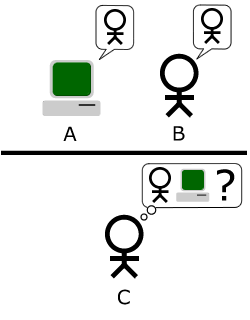
\includegraphics[scale=0.45]{figuras/Turing_Test.png}
    \caption{\tiny{Teste de Turing}}
\end{figure}
\end{columns}
\end{frame}

\begin{frame}{Aprendizado profundo (``Deep Learning'')}
\begin{figure}
    \centering
    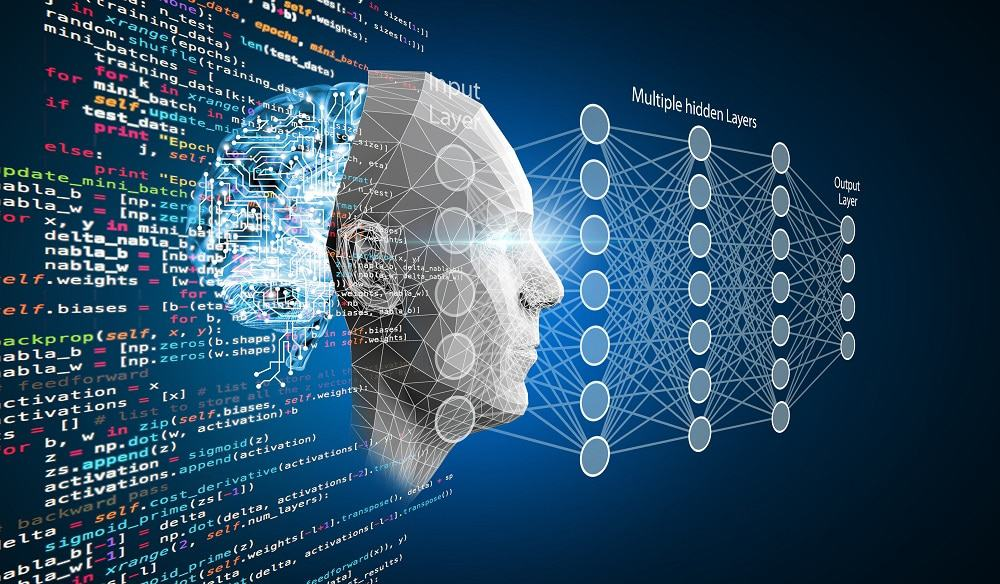
\includegraphics[scale=0.35]{figuras/deep-learning.jpg}
\end{figure}
\end{frame}



\begin{frame}{Deep Learning}
\begin{itemize}
\item Avanço significativo nas redes neurais profundas.
\begin{figure}
    \centering
    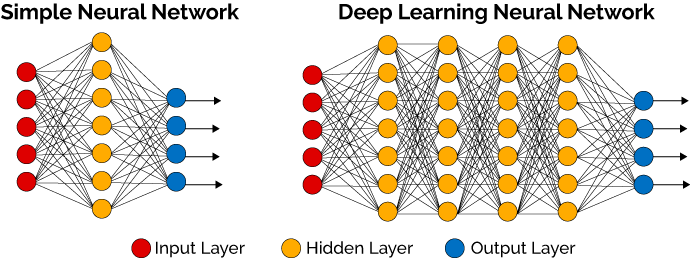
\includegraphics[scale=0.4]{figuras/neural.png}
\end{figure}
\item Melhoria no processamento de grandes volumes de dados.
\item Impulsionou o desenvolvimento de modelos de IA como o ChatGPT.
\end{itemize}
\end{frame}


\begin{frame}{Origem do ChatGPT}
\begin{itemize}
\item ChatGPT é baseado na arquitetura GPT (Transformador de Pré-Treinamento Generativo).
\item Desenvolvido pela OpenAI em 2020.
\item Uso de grandes quantidades de texto para treinamento.
\end{itemize}
\begin{figure}
    \centering
    
\includegraphics[scale=0.4]{figuras/chatboot.png}
\end{figure}
\end{frame}

\begin{frame}{Funcionamento do ChatGPT}
\begin{itemize}
\item ChatGPT é um modelo de linguagem baseado em IA.
\item Capaz de responder a perguntas e gerar texto coerente.
\item Treinado em uma variedade de tópicos e idiomas.
\end{itemize}
\begin{figure}
    \centering
    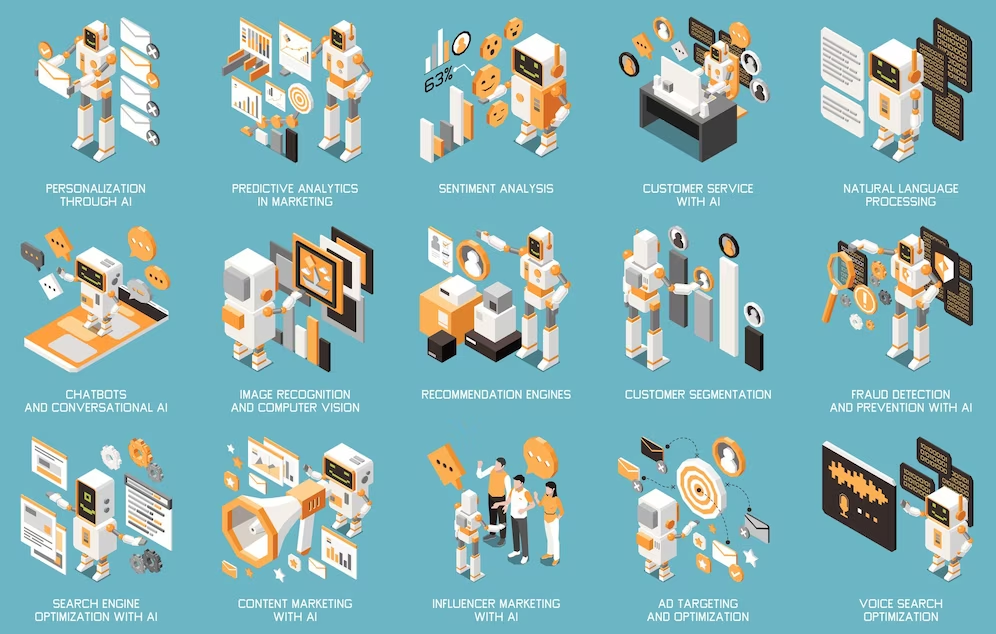
\includegraphics[scale=0.35]{figuras/funcoes.png}
\end{figure}
\end{frame}

\begin{frame}{Prompts para ChatGPT}
\begin{block}{Prompts positivos}
Comandos que orientam o ChatGPT a fornecer informações relevantes para a geração do diálogo ou texto.\\
EX.: ``Escreva um tópico sobre os benefícios da inteligência artificial para as empresas''
\end{block}
\pause
\begin{block}{Prompts negativos}
Comandos que orientam o ChatGPT informa apenas informações relevantes para a geração do diálogo ou texto.\\
EX.: ``Não inclua informações sobre religião e política na sua resposta''
\end{block}

\pause
\begin{block}{Prompts de tarefas}
Comandos que orientam o ChatGPT para realizar determinada tarefa.\\
EX.: ``Crie um gráfico ggplot2 utilizando a linguagem R''
\end{block}

\end{frame}

\section{Uso prático do ChatGPT}
\begin{frame}{Uso prático}
\begin{itemize}\itemsep=2cm
    \item Façam login no ChatGPT (\url{https://chat.openai.com/})
    \item Faça uma pergunta qualquer no ChatGPT.
\end{itemize}
\end{frame}

\begin{frame}{Amor entre o Jubileu e um ET}
\begin{itemize}\itemsep=2cm
    \item Peça ao ChatGPT escrever uma música sobre a história de amor entre o Jubileu e um ET.
\end{itemize}
\end{frame}

\begin{frame}{Traduzir texto para o português}
 \textcolor{blue}{In plant cells, mitochondria play a central role in energy production through the process of cellular respiration, converting organic molecules into adenosine triphosphate (ATP), which is essential to fuel a variety of intracellular functions. In addition, they are involved in regulatory and antioxidant functions, adjusting their activity to tolerant conditions and participating in the synthesis of crucial molecules such as amino acids and lipids. In summary, mitochondria are pivotal in plant cells, ensuring an energy supply and contributing to vital regulatory functions for healthy cellular activity.}
\end{frame}


\begin{frame}{Destacando ideias principais de texto}
 \textcolor{blue}{For over a century, ecotoxicological studies have reported the occurrence of hormesis as a significant phenomenon in many areas of science. In plant biology, hormesis research focuses on measuring morphological, physiological, biochemical, and productivity changes in plants exposed to low doses of herbicides. These studies involve multiple features that are often correlated. However, the multivariate aspect and interdependencies among components of a plant system are not considered in the adopted modeling framework. Therefore, a multivariate nonlinear modeling approach for hormesis is proposed, where information regarding correlations among response variables is taken into account through a variance-covariance matrix obtained from univariate residuals...}
\end{frame}

\begin{frame}{Escrever um texto/corrigir texto}
\begin{itemize}\itemsep=1cm
    \item Sobre a função das mitocôndrias nas células vegetais, com dois parágrafos.
    \pause
    \item Peça para ele resumir o texto para apenas um parágrafo.
    \pause
    \item Diga ao ChatGPT que vai mudar de assunto e peça para ele escrever um pequeno texto com erros ortográficos.
\end{itemize}
\end{frame}

\begin{frame}{Criando um texto para o Instagram}

Peça para o ChatGPT escrever uma postagem da III SITEC com máximo 100 palavras.

\begin{figure}
\centering

\includegraphics[scale=0.1]{figuras/instagram.jpeg}
\end{figure}

 \textcolor{blue}{A III Semana Integrada de Tecnologia, Ciência e Cultura está de volta e mais importante do que nunca! Este evento incrível reúne mentes brilhantes, promovendo a inovação e o diálogo interdisciplinar. É uma oportunidade única para explorar o futuro da tecnologia, a profundidade da ciência e a riqueza da cultura. Junte-se a nós para aprender, inspirar-se e colaborar. Juntos, podemos moldar um mundo mais conectado e criativo. Não perca!}
 

\end{frame}



%--slide
\begin{frame}{Resolvendo um problema de matemática}
\begin{itemize}\itemsep=1cm
    \item Resolva a seguinte equação $f(x)=3x-3=0$.
    \pause
    \item Resolva a seguinte equação $f(x)=x^2=0$.
    \item Resolva a seguinte integral $\int_{1}^{2} x^2 \, dx
$.
\end{itemize}
\end{frame}


\section*{}
\begin{frame}
\begin{center}
\begin{huge}
Muito Obrigado! 
\end{huge} \\
\faEnvelope\space deocleciojardim@hotmail.com 
\end{center}
\hyperlink{pgini}{\beamerreturnbutton{Home page}}
\end{frame}




\end{document}




